\begin{figure*}[t]
\centering
\begin{minipage}{0.54\textwidth}
\centering
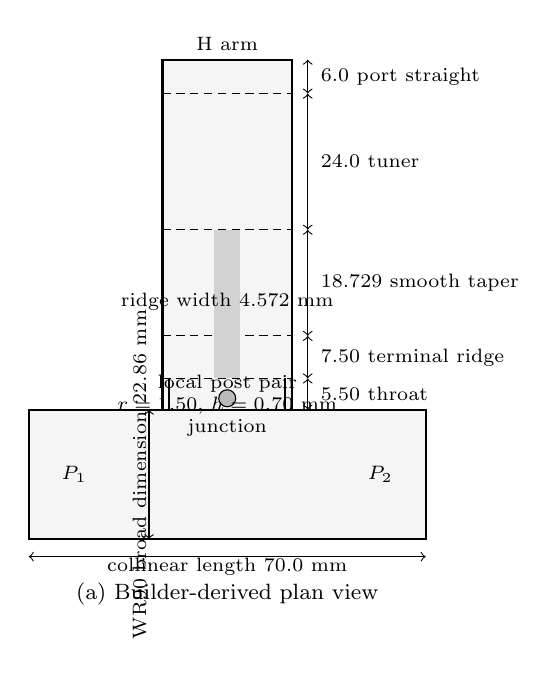
\begin{tikzpicture}[x=0.072cm,y=0.072cm]
% Actual plan-view dimensions from the builder.
\fill[gray!8] (-35,-11.43) rectangle (35,11.43);
\draw[thick] (-35,-11.43) rectangle (35,11.43);
\fill[gray!8] (-11.43,11.43) rectangle (11.43,73.159);
\draw[thick] (-11.43,11.43) rectangle (11.43,73.159);

% H-arm longitudinal section boundaries.
\foreach \yy in {16.93,24.43,43.159,67.159} {
  \draw[densely dashed] (-11.43,\yy) -- (11.43,\yy);
}

% Reduced-width throat.
\draw[thick] (-10.2,11.43) -- (-10.2,16.93);
\draw[thick] (10.2,11.43) -- (10.2,16.93);

% Centerline ridge footprint from terminal section through taper.
\fill[gray!35] (-2.286,16.93) rectangle (2.286,43.159);

% Local partial-height post pair location (plan footprint).
\draw[fill=gray!55] (0,13.43) circle (1.5);

% Dimension arrows for H-arm sections.
\draw[<->] (14.2,11.43) -- (14.2,16.93);
\node[font=\scriptsize,anchor=west] at (14.8,14.18) {5.50 throat};
\draw[<->] (14.2,16.93) -- (14.2,24.43);
\node[font=\scriptsize,anchor=west] at (14.8,20.68) {7.50 terminal ridge};
\draw[<->] (14.2,24.43) -- (14.2,43.159);
\node[font=\scriptsize,anchor=west] at (14.8,33.79) {18.729 smooth taper};
\draw[<->] (14.2,43.159) -- (14.2,67.159);
\node[font=\scriptsize,anchor=west] at (14.8,55.16) {24.0 tuner};
\draw[<->] (14.2,67.159) -- (14.2,73.159);
\node[font=\scriptsize,anchor=west] at (14.8,70.16) {6.0 port straight};

% Main labels.
\node[font=\scriptsize] at (-27,0) {$P_1$};
\node[font=\scriptsize] at (27,0) {$P_2$};
\node[font=\scriptsize] at (0,76.0) {H arm};
\node[font=\scriptsize,align=center] at (0,8.2) {junction};
\node[font=\scriptsize,align=center] at (0,14.0) {local post pair\\$r=1.50$, $h=0.70$ mm};
\node[font=\scriptsize] at (0,30.5) {ridge width $4.572$ mm};

% Overall WR90 dimensions.
\draw[<->] (-35,-14.5) -- (35,-14.5);
\node[font=\scriptsize] at (0,-16.2) {collinear length $70.0$ mm};
\draw[<->] (-13.8,-11.43) -- (-13.8,11.43);
\node[font=\scriptsize,rotate=90] at (-15.5,0) {WR90 broad dimension $22.86$ mm};

\node[font=\footnotesize] at (0,-21.0) {(a) Builder-derived plan view};
\end{tikzpicture}
\end{minipage}\hfill
\begin{minipage}{0.43\textwidth}
\centering
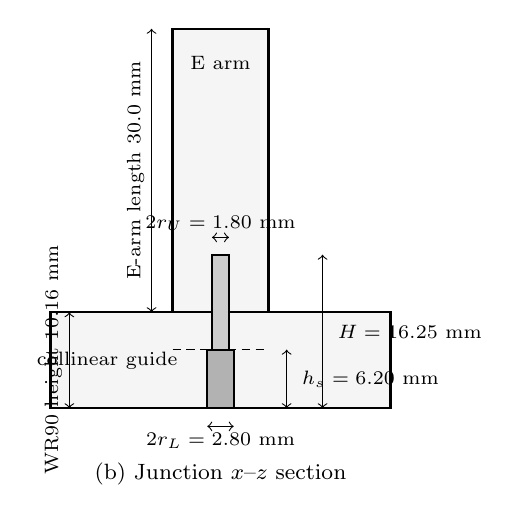
\begin{tikzpicture}[x=0.12cm,y=0.12cm]
% x-z junction section using actual final post dimensions.
\fill[gray!8] (-18,-5.08) rectangle (18,5.08);
\draw[thick] (-18,-5.08) rectangle (18,5.08);

% E arm: width B in x, length 30 mm above the WR90 top wall.
\fill[gray!8] (-5.08,5.08) rectangle (5.08,35.08);
\draw[thick] (-5.08,5.08) rectangle (5.08,35.08);

% Final stepped post.
\fill[gray!60] (-1.40,-5.08) rectangle (1.40,1.12);
\draw[thick] (-1.40,-5.08) rectangle (1.40,1.12);
\fill[gray!40] (-0.90,1.12) rectangle (0.90,11.17);
\draw[thick] (-0.90,1.12) rectangle (0.90,11.17);

% Split and total-height annotations.
\draw[densely dashed] (-5.08,1.12) -- (5.08,1.12);
\draw[<->] (7.0,-5.08) -- (7.0,1.12);
\node[font=\scriptsize,anchor=west] at (7.6,-1.98) {$h_s=6.20$ mm};
\draw[<->] (10.8,-5.08) -- (10.8,11.17);
\node[font=\scriptsize,anchor=west] at (11.4,3.05) {$H=16.25$ mm};

\draw[<->] (-1.40,-7.0) -- (1.40,-7.0);
\node[font=\scriptsize] at (0,-8.5) {$2r_L=2.80$ mm};
\draw[<->] (-0.90,13.0) -- (0.90,13.0);
\node[font=\scriptsize] at (0,14.5) {$2r_U=1.80$ mm};

% E-arm length.
\draw[<->] (-7.3,5.08) -- (-7.3,35.08);
\node[font=\scriptsize,rotate=90] at (-9.0,20.08) {E-arm length $30.0$ mm};

% Waveguide height.
\draw[<->] (-16,-5.08) -- (-16,5.08);
\node[font=\scriptsize,rotate=90] at (-17.7,0) {WR90 height $10.16$ mm};

\node[font=\scriptsize] at (0,31.5) {E arm};
\node[font=\scriptsize] at (-12,0) {collinear guide};
\node[font=\footnotesize] at (0,-12.0) {(b) Junction $x$--$z$ section};
\end{tikzpicture}
\end{minipage}

\caption{Dimensioned layout of the actual single-cell model used for the full-wave identification, reconstructed directly from the geometry builder and the final nominal stepped-post parameters. The H arm contains a 5.50-mm reduced-width throat, a 7.50-mm terminal ridge section, an 18.729-mm smooth two-section ridge taper, a 24.0-mm tuner straight, and a 6.0-mm reference-port straight. The junction section shows the final lower radius $r_L=1.40$~mm, split height $h_s=6.20$~mm, upper radius $r_U=0.90$~mm, and total post height $H=16.25$~mm. This figure is dimensioned from the simulation builder rather than drawn as a conceptual schematic.}
\label{fig:dimensioned-design}
\end{figure*}
